
\section{Límites}

\begin{itemize}	
	\item Consideramos la función de $\R$ en $\R$ definida por $1 + x^2$ para $x > 0$ y $1 - x^2$ para $x < 0$. 
	\item El gráfico de la función es como sigue: 
	\begin{center}
		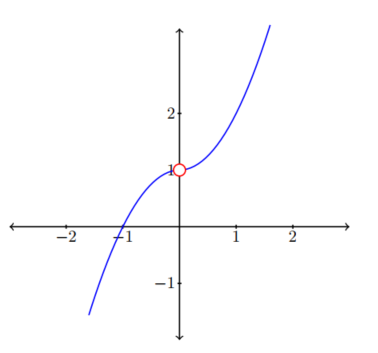
\includegraphics[scale=0.5]{figuras/capitulo1/04-limites/intro.png}
	\end{center}
	\item Esta función no está definida en $x=0$, sin embargo, cuando se consideran valores de $x$ no nulos, pero cercanos a 0, los valores de $f(x)$ se aproximan a $1$. 
	\item Lo anterior corresponde a la idea intuitiva de que los valores de $f(x)$ tienden a 1 cuando $x$ tiende a 0. 
	\item Lo que queremos hacer es formalizar esta intuición. 
	\item Referencia: Apunte Introducción al Cálculo, semanas 9, 12 y 13. 
\end{itemize}

	Antes de definir la noción de límite, necesitaremos hacer uso de otro concepto matemático de relevancia: 

\begin{definicion}
	\textbf{(Sucesión)}
	Una \textbf{sucesión} real es una función $f: \N \rightarrow \R$. 
\end{definicion}
 
\begin{nota}
	\textbf{Notación:} En lugar de utilizar la notación habitual de las funciones, las sucesiones se denotan por $(s_n)$ o $(s_n)_{n\in\N}$.  
\end{nota}

\begin{definicion}
	\textbf{(Convergencia de sucesiones)}
	Diremos que la sucesión $(s_n)$ converge a $l$ o bien que los términos $s_n$ tienden a $l$, lo que denotamos por $s_n \rightarrow l$ si se cumple que: 
	$$ \forall \varepsilon > 0, \exists n_0 \in \N, \forall n \geq n_0, \quad s_n \in [l - \varepsilon, l + \varepsilon] $$
\end{definicion}

\begin{nota}
	En el concepto de la topología (que veremos más adelante en el curso), el intervalo $ [l - \varepsilon, l + \varepsilon]$ suele llamarse \textbf{vecindad} en torno a $l$. 
\end{nota}


\begin{ejemplo}
	Veamos que la sucesión $(s_n)$ definida por $s_n = \frac{1}{n}$ converge a $0$.  
\end{ejemplo}

\begin{itemize}
	\item Debemos mostrar que: 
	$$ \forall \varepsilon > 0, \exists n_0 \in \N, \forall n \geq n_0, \quad \frac{1}{n} \in [- \varepsilon, \varepsilon] $$
	\item Notemos que $\frac{1}{n} \in [- \varepsilon, \varepsilon]$ equivale a imponer que: 
	$$ | \frac{1}{n} | < \varepsilon $$ 
	\item Como $\frac{1}{n}>0$, lo anterior es equivalente a que: 
	$$ \frac{1}{n} < \varepsilon \quad \iff \quad n \geq \frac{1}{\varepsilon}$$ 
	\item Luego, dado $\varepsilon > 0$, basta tomar $n_0 = \left[\dfrac{1}{\varepsilon}\right] + 1$ y se tendrá que para todo $n \geq n_0$: 
	$$  n \geq \frac{1}{\varepsilon} $$ 
\end{itemize}

La noción de límite en sucesiones será de utilidad para analizar el límite de funciones de variable real. 

\bigskip 	
Sin embargo, para formalizar el concepto necesitamos introducir un concepto más: 

\begin{definicion}{\textbf{Punto de acumulación}}
	Sea $A \subseteq \R$ un subconjunto cualquiera de $\R$. El real $\bar{x}\in \R$ se dirá \textbf{punto de acumulación} de  $A$ si existe alguna sucesión $(x_n) \subseteq A$ tal que $x_n \neq \bar{x}, \forall n \geq n_0$, algún $n_0$ y $x_n \rightarrow \bar{x}$. 
\end{definicion}

El conjunto de todos los puntos de acumulación de $A\subseteq \R$ se denota por $A'$. 


\begin{observacion}
	En general, $A$ no está contenido en $A'$. Por ejemplo, para $ A = (0, 1) \cup \{2\}$, $A' = [0,1]$. 
\end{observacion}

\begin{definicion}
	\textbf{(Límite de funciones)}
	Sea $f : A \subseteq \R \longrightarrow \R$ y sea $\bar{x} \in A'$, es decir, $\bar{x}$ es un punto de acumulación de $A$. Diremos que $f$ tiende a $l\in \R$ cuando $x$ tiende a $\bar{x}$ (lo que denotamos $f(x)\rightarrow l$ cuando $x\rightarrow \bar{x}$) o bien que $l$ es el \textbf{límite} de $f(x)$ cuando $x\rightarrow \bar{x}$ (lo que se anota $l = lim_{x\rightarrow\bar{x}} f(x)$) si para toda sucesión $(x_n)$ con valores en $A$, convergente a $\bar{x}$ y tal que $x_n \neq \bar{x}$, se cumple que la sucesión de las imágenes $(f(x_n))$ es convergente a $l$. 
\end{definicion}

\begin{observacion}
	\begin{itemize}
		\item Si $\bar{x}\notin A$, entonces no existen sucesiones $(x_n)$ con valores en $A \setminus\{\bar{x}\}$ convergentes a $\bar{x}$, luego no puede estudiarse el límite de la función cuando $x \rightarrow \bar{x}$.  
		\item Si $\bar{x}\in A'$, entonces el concepto de límite está bien definido, aunque podría no existir. 
	\end{itemize}
\end{observacion}


\begin{ejemplo}
	\begin{itemize}
		\item $lim _{x\rightarrow 1} \dfrac{x^2 - 1}{x-1} = 2$. 
		\item $\lim_{x\rightarrow -1} \sqrt{x}$ no existe, ya que $-1 \notin (R^+ \cup \{0\})'$. 
		\item $lim_{x\rightarrow 0} \dfrac{1}{x}$ no existe, ya que por ejemplo $x_n = \frac{1}{n} \rightarrow 0$, pero $\frac{1}{x_n} = n$ no converge. 
	\end{itemize}
\end{ejemplo}


\begin{teorema}
	\textbf{(Unicidad del límite)}
	Si una función $f$ tiene límite cuando $x\rightarrow \bar{x}$, entonces dicho límite es único. 
\end{teorema}

\begin{proof}
	Sean $l_1$ y $l_2$ límites de $f(x)$ cuando $x\rightarrow \bar{x}$. Sea entonces $(x_n)$ alguna sucesión con valores en el dominio de la función $f$ y convergente a $\bar{x}$. Entonces, por definición de límite se tiene que la sucesión es convergente a $l_1$ y a $l_2$ simultáneamente. Gracias al teorema de unicidad para el límite de sucesiones, se tiene que $l_1 = l_2$. 
\end{proof}

\begin{teorema}
	\textbf{(Álgebra de límites)}
	Sean $f$ y $g$ dos funciones y $\bar{x}\in \R$ tales que $ \lim_{x\rightarrow\bar{x}} f(x) = l_1$ y $\lim_{x\rightarrow\bar{x}}g(x) = l_2$. Entonces: 
	\begin{itemize}
		\item Si $\bar{x} \in (Dom(f))' \cap (Dom(g))'$, se tiene que: 
		$$ \lim_{x\rightarrow\bar{x}}(f+g)(x) = l_1 + l_2 $$ 
		$$ \lim_{x\rightarrow\bar{x}}(f-g)(x) = l_1 - l_2 $$ 
		$$ \lim_{x\rightarrow\bar{x}}(fg)(x) = l_1  l_2 $$ 
		\item Si $\bar{x} \in (Dom(f/g))'$ y $l_2 \neq 0$, entonces: 
		$$ \lim_{x\rightarrow\bar{x}} (f/g)(x) = l_1/l_2 $$ 
		\item En particular (cuando $g$ es constante), se tiene que, $\forall \alpha \in \R$: 
		$$ \lim_{x\rightarrow\bar{x}} (\alpha f ) (x) = \alpha l_1 $$ 
	\end{itemize}
\end{teorema}

\begin{teorema}
	\textbf{(Sandwich)}
	Sean $f, g$ y $h$ funciones y sea $\bar{x} \in (Dom(g))'$. 
	Si $\exists \delta > 0, \forall x \in Dom(g) \cap [\bar{x} - \delta , \bar{x} + \delta ] f(x) \leq g(x) \leq h(x) $, y además $\lim_{x\rightarrow\bar{x}} f(x) = \lim_{x\rightarrow\bar{x}} h(x) = l$, entonces: 
	$$ \lim_{x\rightarrow\bar{x}} g(x) = l $$ 
\end{teorema}
